\documentclass{beamer}
\usepackage[utf8]{inputenc}
\usepackage{amsmath,amsfonts,amsthm,amstext,amssymb, xcolor, tikz, pgf}
\usepackage{stmaryrd}
% ----------------------------------------------------------
% Theme Setup

% Use Metropolis Theme
\usetheme[numbering=fraction]{metropolis}
\setbeamertemplate{blocks}[rounded][shadow=false]
\makeatletter
\setlength{\metropolis@titleseparator@linewidth}{1pt}
\makeatother

% Define Colors
\definecolor{chargerblue}{HTML}{002764}
\definecolor{chargerred}{HTML}{e02034}
\definecolor{bggray}{HTML}{d0d3d4}

% Set Colors
\setbeamercolor{title}{fg=chargerblue}
\setbeamercolor{background canvas}{bg=white}
\setbeamercolor{title separator}{fg=chargerred}
\setbeamercolor{structure}{fg=chargerblue}
\setbeamercolor{frametitle}{fg=white, bg=chargerblue}
\setbeamercolor*{normal text}{fg=chargerblue}
\setbeamercolor*{block body}{bg=bggray}
\setbeamercolor*{block title}{bg=chargerblue, fg=white}
% ----------------------------------------------------------

% ----------------------------------------------------------
% Custom Definitions, Commands, Environments, etc.

% Sets of numbers
\def\R{\mathbb{R}} % The reals
\def\N{\mathbb{N}} % The naturals
\def\Z{\mathbb{Z}} % The integers
\def\Q{\mathbb{Q}} % The rationals

% Blank space
\newcommand{\blank}[1]{\underline{\hspace{#1}}} % Blank space

% Fitted inclusion symbols
\newcommand{\fp}[1]{\left({#1}\right)} % Fitted parentheses around content
\newcommand{\fb}[1]{\left[{#1}\right]} % Fitted brackets
\newcommand{\set}[1]{\left\{{#1}\right\}} % Fitted braces (useful for sets)
\newcommand{\av}[1]{\left|{#1}\right|} % Fitted absolute value bars



% Coordinate Plane (Four-Quadrant)
\def\coordplane {
	\begin{tikzpicture}		\draw[step=0.25cm,black,very thin,opacity=0.25] (-2.5cm, -2.5cm) grid (2.5cm, 2.5cm);
		\draw[<->,thick,black] (-2.5cm, 0) -- (2.5cm, 0) node[anchor=north west,pos=0.94,font=\scriptsize]{$x$};
		\draw[<->,thick,black] (0,-2.5cm) -- (0, 2.5cm) node[anchor=south east,font=\scriptsize,pos=0.94]{$y$};
	\end{tikzpicture}
}

% Coordinate Plane (One-Quadrant)
\def\onequad {
	\begin{tikzpicture}
		\draw[step=0.25cm, black, very thin, opacity=0.25] (0,0) grid (7.5cm,5cm);
		\draw[->, thick, black] (0,0) -- (7.5cm, 0) node[anchor=north west,font=\scriptsize,pos=0.94]{$x$};
		\draw[->, black, thick] (0,0) -- (0,5cm) node[anchor=south east,font=\scriptsize,pos=0.94]{$y$};
	\end{tikzpicture}
}
% ----------------------------------------------------------

% ----------------------------------------------------------
% Presentation Information 
\title[2.3-2.5]{Graphs of Functions; Parent Functions and Transformations}
\subtitle{Sections 2.3-2.5}
\author{Jacob Ayers}
\institute{Lesson \#9}
\date{MAT 130}
% ----------------------------------------------------------

\begin{document}

% Slide 1 (Title Slide)
\begin{frame}
\titlepage
\end{frame}

% Slide 2 (Objectives)
\begin{frame}[t]{Objectives}
\begin{itemize}
	\item Find the zeros of a function
	\item Determine intervals on which functions are increasing and decreasing
	\item Find relative minima and maxima of functions
	\item Identify even and odd functions
	\item Recognize graphs of parent functions
	\item Describe transformations of parent functions
\end{itemize}
\end{frame}

\begin{frame}[t]{The Graph of a Function}
\begin{block}{Definition}
The \textit{graph} of a function is the set of all ordered pairs $(x, f(x))$ such that $x$ is in the domain of $f(x)$.
\end{block}

Today's lesson focuses on characteristics of functions' graphs.
\end{frame}

\begin{frame}[t]{Zeros of a Function}
The \textit{zeros} of a function are $x$-values for which $f(x) = 0$.

\pause Graphically, they are the $x$-intercepts of the function.

\pause To find them, $f(x) = 0$ and solve.

\pause Example: Find the zeros of the function $f(x) = 3x^2 + x - 10$.
\pause \begin{flalign*}
3x^2 + x - 10 &= 0 & \\
(3x - 5)(x+2) &= 0 & \\
x &= \set{-2, \dfrac53}
\end{flalign*}
\pause The zeros of the function are $x = -2$ and $x = \dfrac53$
\end{frame}

\begin{frame}[t]{Zeros of a Function}
Find the zeros of the function $h(x) = \dfrac{x^2 - 2}{x-1}$

\begin{flalign*}
\onslide<2->{\dfrac{x^2 - 2}{x-1} &= 0 & \\}
\onslide<3->{x^2 - 2 &= 0 & \\}
\onslide<4->{x^2 &= 2 & \\}
\onslide<5->{x &= \pm \sqrt{2}}
\end{flalign*}
\onslide<6>{The zeros of the function are $x = -\sqrt{2}$ and $x = \sqrt{2}$}
\end{frame}
\begin{frame}[t]{Increasing and Decreasing Functions}
\begin{block}{Increasing, Decreasing, and Constant}
Increasing: A function is \textit{increasing} on an interval if its graph is rising on the interval

Decreasing: A function is \textit{decreasing} on an interval if its graph is falling on the interval

Constant: A function is \textit{constant} on an interval if its graph is flat on that interval
\end{block}

\pause

To determine intervals on which a function is increasing, decreasing, and constant, look for places on its graph where it is rising, falling, and flat.
\end{frame}

\begin{frame}[t]{Increasing and Decreasing Functions}
\begin{columns}
\begin{column}{0.5\textwidth}
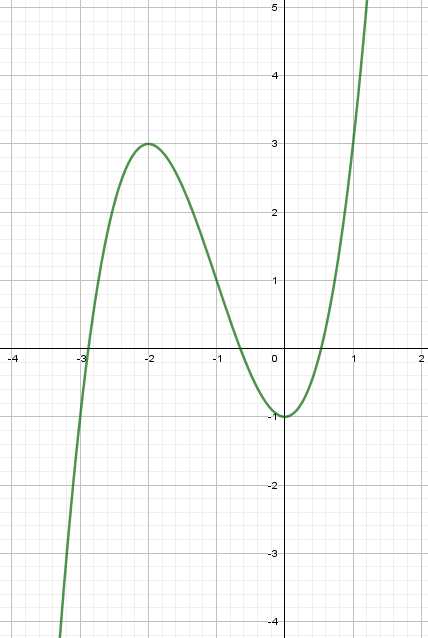
\includegraphics[width=\textwidth]{Graph1.png}
\end{column}
\begin{column}{0.5\textwidth}
Look at the graph, and determine the intervals on which it is increasing, decreasing, or constant. \vspace{12pt}

\pause Increasing: $(\infty, 2) \cup (0, \infty)$ \vspace{12pt}

\pause Decreasing: $(-2, 0)$ \vspace{12pt}

\pause Constant: There are no intervals on which the interval is constant
\end{column}
\end{columns}
\end{frame}

\begin{frame}{Increasing and Decreasing Functions}
\begin{columns}
\begin{column}{0.5\textwidth}
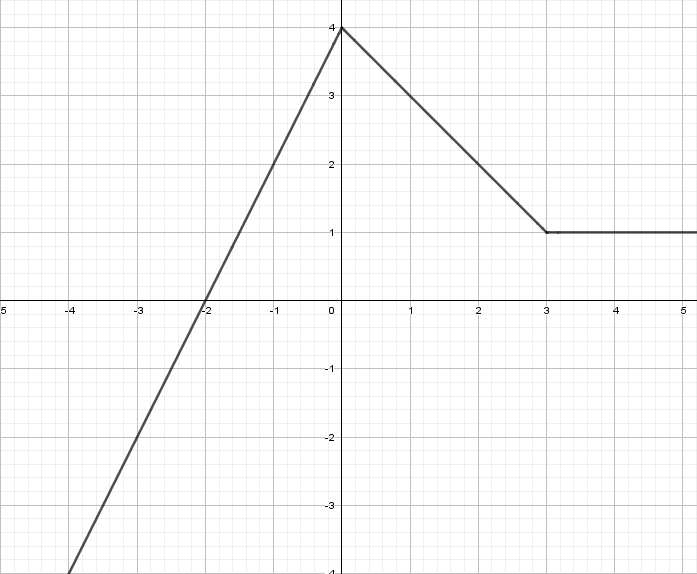
\includegraphics[width=\textwidth]{Graph2.png}
\end{column}
\begin{column}{0.5\textwidth}
Look at the graph, and determine the intervals on which it is increasing, decreasing, or constant. \vspace{12pt}

\pause Increasing: $(-\infty, 0)$ \vspace{12pt}

\pause Decreasing: $(0, 3)$ \vspace{12pt}

\pause Constant: $(3, \infty)$
\end{column}
\end{columns}
\end{frame}

\begin{frame}[t]{Relative Minima and Maxima}
\begin{block}{Definition}
A function value $f(a)$ is a relative minimum of $f$ when there exists an interval $(x_1,x_2)$ that contains $a$ such that $$x_1 < x < x_2 \text{ implies } f(a) \leq f(x)$$

A function value $f(a)$ is a relative maximum of $f$ when there exists an interval $(x_1,x_2)$ that contains $a$ such that $$x_1 < x < x_2 \text{ implies } f(a) \geq f(x)$$
\end{block}

\pause

Put simply: \\
Relative minima are ``bottoms of valleys" of a function's graph \\
Relative maxima are ``tops of hills" of a functions graph

\end{frame}

\begin{frame}[t]{Relative Minima and Maxima}
Use a graphing utility to approximate the relative maximum of the function $f(x) = -4x^2 - 7x + 3$.

I'll demonstrate using GeoGebra. Graphing calculators such as the TI-84 Plus and Casio fx-9750 G-II can also do this; I will try to find videos on YouTube showing you how to use a graphing calculator to approximate extrema.
\end{frame}

\begin{frame}[t]{Even and Odd Functions}
We saw symmetry back in Chapter 1.

\begin{block}{Definition}
A function is \textit{even} if it symmetric about the $y$-axis.

A function is \textit{odd} if it is symmetric about the origin.
\end{block}

\pause

\begin{block}{Test for Even and Odd Functions}
A function $y = f(x)$ is even if $f(-x) = f(x)$ for all $x$ in the domain.

A function $y = f(x)$ is odd if $f(-x) = -f(x)$ for all $x$ in the domain.
\end{block}

\pause

NOTE: It is possible for a function to be neither even nor odd.
\end{frame}

\begin{frame}[t]{Even and Odd Functions}
Determine whether $f(x) = x^4 - x^2 - 1$ is even, odd or neither.
\begin{flalign*}
\onslide<2->{f(-x) &= (-x)^4 - (-x)^2 - 1 & \\}
\onslide<3->{&= x^4 - x^2 - 1 & \\}
\onslide<4->{&= f(x) \Rightarrow f(x) \text{ is even}}
\end{flalign*}

Determine whether $f(x) = 2x^3 + 3x$ is even, odd, or neither.
\begin{flalign*}
\onslide<5->{f(-x) &= 2(-x)^3 + 3(-x) & \\}
\onslide<6->{&= -2x^3 - 3x & \\}
\onslide<7->{&= -(2x^3 + 3x) & \\}
\onslide<8>{&= -f(x) \Rightarrow f(x) \text{ is odd} &}
\end{flalign*}
\end{frame}

\begin{frame}[t]{Parent Functions - The Identity Function}
Function Notation: $f(x) = x$

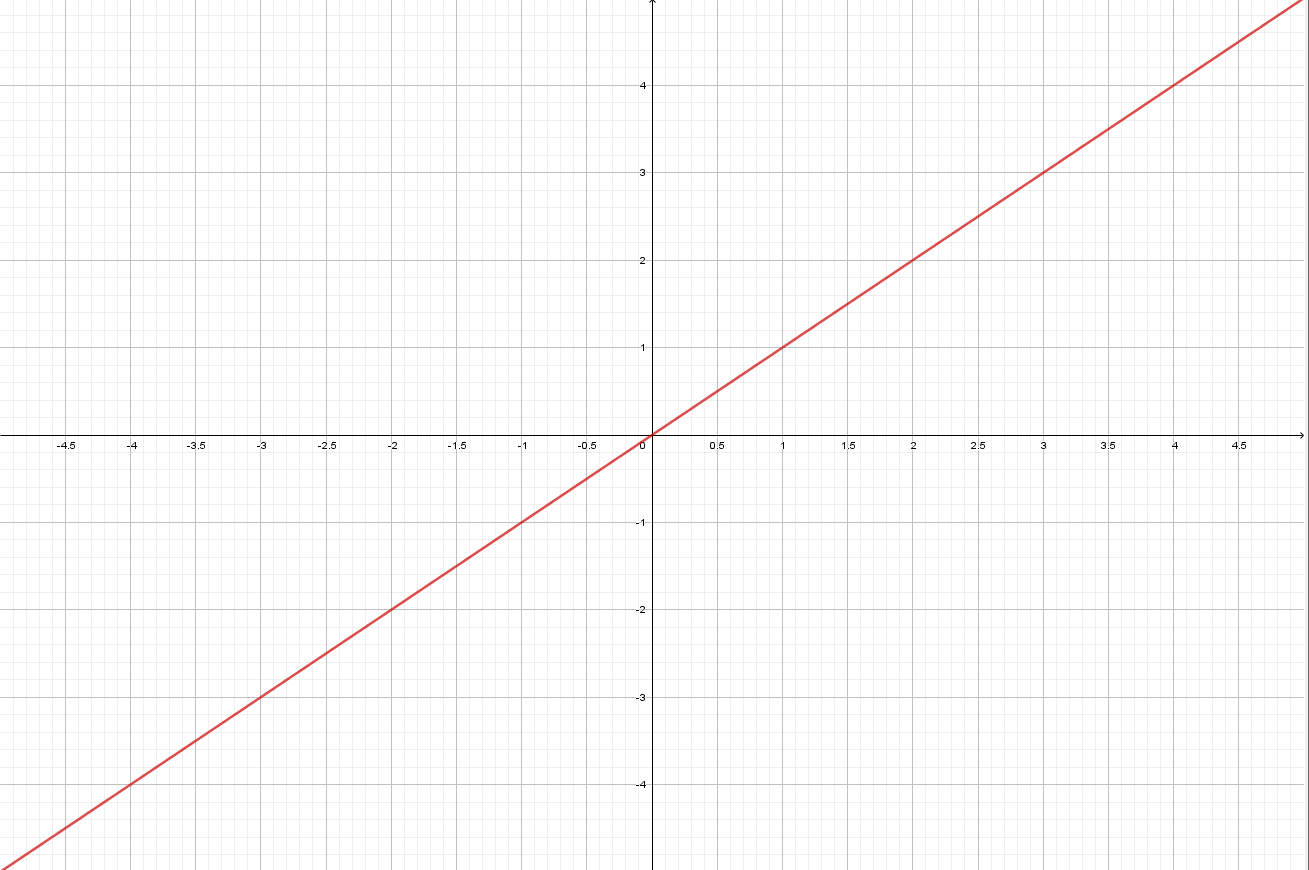
\includegraphics[width=\textwidth]{Identity.png}
\end{frame}

\begin{frame}[t]{Parent Functions - The Squaring Function}
Function Notation: $f(x) = x^2$

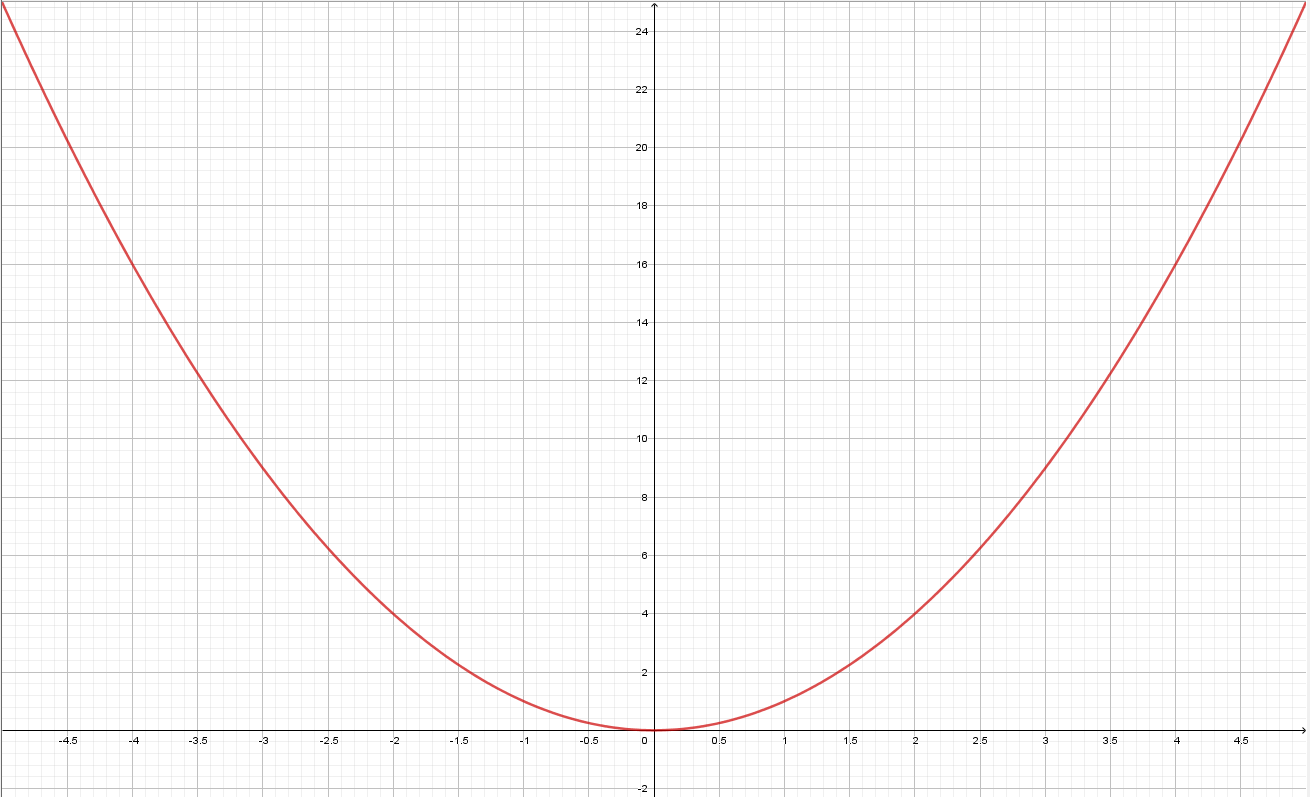
\includegraphics[width=\textwidth]{Squaring.png}
\end{frame}

\begin{frame}[t]{Parent Functions - Cubic Function}
Function Notation: $f(x) = x^3$

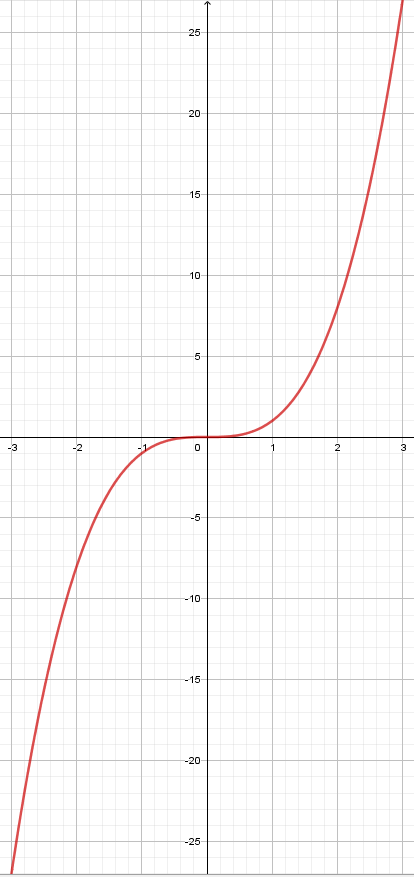
\includegraphics[scale=0.25]{Cubic.png}
\end{frame}

\begin{frame}[t]{Parent Functions - Square Root Function}
Function Notation: $f(x) = \sqrt{x}$

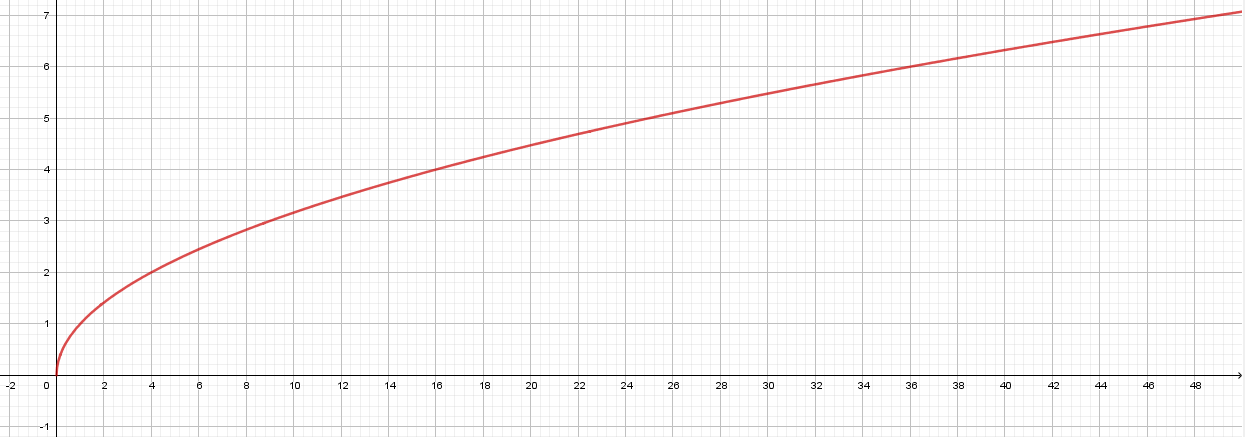
\includegraphics[width=\textwidth]{SQRT.png}
\end{frame}

\begin{frame}[t]{Parent Functions - Step Function}
Function Notation: $f(x) = \llbracket x \rrbracket$

\pause

The \textit{greatest integer in $x$}, denoted by $\llbracket x \rrbracket$, is the largest integer $y$ such that $y \leq x$.

\pause

Examples: \\
$\llbracket \pi \rrbracket = 3$ \\
$\left\llbracket -\dfrac12 \right\rrbracket = -1$ \\
$\llbracket -7.28 \rrbracket = -8$

\end{frame}

\begin{frame}[t]{Parent Functions - Step Function}
The graph below should show you why we call this function the step function.

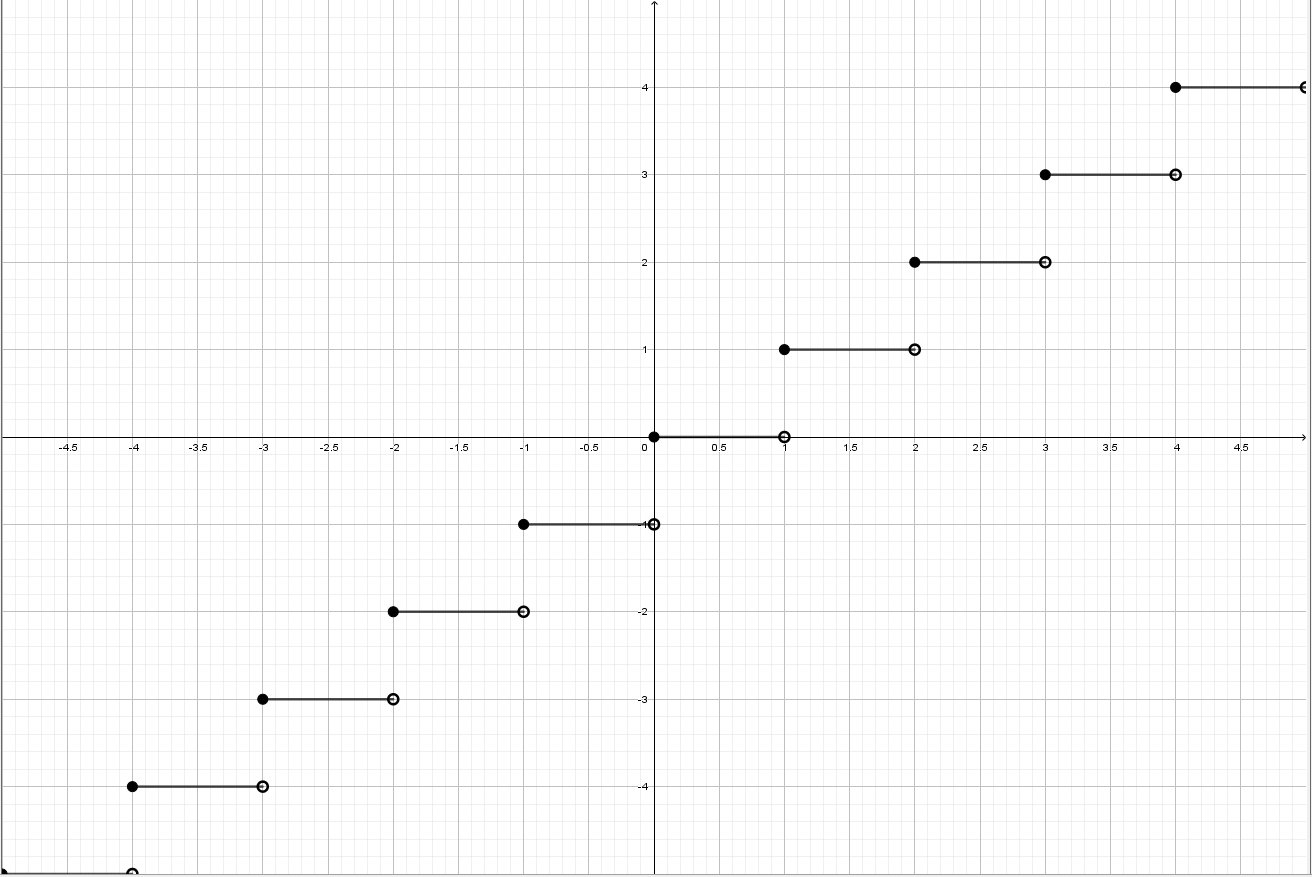
\includegraphics[width=0.8\textwidth]{Step.png}
\end{frame}

\begin{frame}[t]{Shifting Graphs of Functions}
Suppose we have a parent function $y = f(x)$

There are various ``modifications" we can make to the function that will move its graph around. \vspace{18pt}

\pause

The first such modification is a horizontal shift. 

The function $y = f(x-h)$ represents a horizontal shift of $h$ units to the right (or left, if $h$ is negative)
\end{frame}

\begin{frame}[t]{Shifting Graphs of Functions}
Identify the parent function and describe the transformation: \\
$f(x) = \sqrt{x - 3}$

\pause

The parent function is $y = \sqrt{x}$.

\pause

Since $h = 3$, this function is the square root function, shifted 3 units to the right. \vspace{18pt}

\pause

Identify the parent function and describe the transformation: \\
$f(x) = (x+6)^3$

\pause

The parent function is $y = x^3$.

\pause

Since $h = -6$, this function is the cubic function, shifted 6 units to the left.
\end{frame}

\begin{frame}[t]{Shifting Graphs of Functions}
We can also shift a graph vertically.

The function $y = f(x) + k$ represents a vertical shift of $k$ units up (or down, if $k$ is negative). \vspace{12pt}

\pause

Identify the parent function and describe the transformation: \\
$f(x) = \llbracket x \rrbracket - 8$

\pause

The parent function is $y = \llbracket x \rrbracket$.

\pause

Since $k = -8$, this function is the step function, shifted 8 units down. 
\end{frame}

\begin{frame}[t]{Shifting Graphs of Functions}
Identify the parent function and describe the transformation: \\
$f(x) = x + 11$

\pause

The parent function is $y = x$.

\pause

Since $k = 11$, this function is the identity function, shifted 11 units up. \vspace{18pt}

Identify the parent function and describe the transformation: \\
$f(x) = \sqrt{x - 2} + 3$

\pause

The parent function is $y = \sqrt{x}$

\pause

This time, we have values for both $h$ and $k$. Since $h = 2$ and $k = 3$, this function is the square root function, shifted 2 units right and 3 units up.
\end{frame}

\begin{frame}[t]{Reflecting Graphs of Functions}
Think of reflection as a mirror image. There are two types of reflection for a graph:

\pause

1) Reflection across $x$-axis: $h(x) = -f(x)$

2) Reflection across $y$-axis: $h(x) = f(-x)$

\pause

Where the negative sign is is very important!
\end{frame}

\begin{frame}[t]{Reflecting Graphs of Functions}
Identify the parent function and describe the transformation: \\
$f(x) = -x^3$

\pause

The parent function is $y = x^3$

\pause

In this case, we are looking at a modification of the form $y = -f(x)$, so this is a reflection of the cubic function across the $x$-axis. (Note: if it were a reflection across the $y$-axis, it would've been written as $f(x) = (-x)^3$)
\end{frame}

\begin{frame}[t]{Reflecting Graphs of Functions}
Identify the parent function and describe the transformation: \\
$f(x) = \sqrt{-x}$

\pause

The parent function is $f(x) = \sqrt{x}$

Since the negative is under the square root, this is a modification of the form $y = f(-x)$; this is a reflection of the square root function across the $y$-axis.
\end{frame}

\begin{frame}[t]{Putting It Together: Shifting And Reflecting}
Identify the parent function and describe the transformation: \\
$f(x) = (-x + 6)^2 + 5$

\pause

The parent function is $y = x^2$

\pause Determining the tranformation is a little tricky. One thing that is clear is that the graph will be shifted up 5 units. You might guess that it is reflected across the $y$-axis and shifted left 6 units, but that is not the case.

\pause

Note that $(-x+6) = -(x - 6)$, so we can rewrite this function as $f(x) = -(x-6)^2 + 5$, at which point we can easily see that this is a reflection across the $x$-axis and a shift right of 6 units.

\pause

You should use this type of simplification any time you have a function of the form $y = f(-x - h)$.
\end{frame}

\begin{frame}[t]{Next Steps}
\begin{itemize}
\item Post questions in the Lesson 9 Forum, if you have any
\item Read 2.6 and 2.7
\item Watch Video Lesson \#10
\end{itemize}
\end{frame}

\end{document}